% ==============================================================================
%  SUPPLEMENTARY MATERIAL
%  Compile with pdflatex (run twice so cross-references resolve).
% ==============================================================================
\documentclass[11pt]{article}

% ── Page & fonts ─────────────────────────────────────────────────────────────
\usepackage[a4paper, margin=2cm]{geometry}   % use letterpaper if your journal is US-based
\usepackage[T1]{fontenc}
\usepackage[utf8]{inputenc}
\usepackage{lmodern}

% ── Math ─────────────────────────────────────────────────────────────────────
\usepackage{amsmath, amssymb}

% ── Tables ───────────────────────────────────────────────────────────────────
\usepackage{array}        % >{\raggedright\arraybackslash}p{...} columns
\usepackage{booktabs}     % \toprule \midrule \bottomrule
\usepackage{longtable}    % tables that span pages
\usepackage{multirow}
\usepackage{pdflscape}    % landscape pages (rotated in the PDF viewer too)

% ── Figures ──────────────────────────────────────────────────────────────────
\usepackage{graphicx}
\usepackage{xcolor}
\graphicspath{{figures/}{../Python Analysis/final_plot/}}   % edit to your folders
\usepackage{caption}
\captionsetup{font=small, labelfont=bf}

% ── References & links ───────────────────────────────────────────────────────
\usepackage[hidelinks]{hyperref}
% Optional: refer to labels in the main paper, e.g. \ref{fig:methods_overview}.
% Compile the main paper first, then uncomment (main.aux must exist):
% \usepackage{xr-hyper}
% \externaldocument[main-]{../main}   % then use \ref{main-fig:methods_overview}

% ── "S" numbering: Table S1, Figure S1, Eq. (S1), Section S1 ─────────────────
\renewcommand{\thetable}{S\arabic{table}}
\renewcommand{\thefigure}{S\arabic{figure}}
\renewcommand{\theequation}{S\arabic{equation}}
\renewcommand{\thesection}{S\arabic{section}}
\renewcommand{\thepage}{S\arabic{page}}

\begin{document}

% ── Title page ───────────────────────────────────────────────────────────────
\begin{center}
  \thispagestyle{empty}          % no page number on the title page
  \vspace*{\fill}

  {\fontsize{30}{36}\selectfont\bfseries Supplementary Material\par}
  \vspace{0.8cm}
  {\color{gray!60}\rule{0.6\linewidth}{0.8pt}\par}
  \vspace{0.8cm}

  {\Large\bfseries
   Stereoelectroencephalography-Based Functional Connectivity\\[4pt]
   in Drug-Resistant Epilepsy:\\[4pt]
   A Systematic Review of Methods, Reporting Standards,\\[4pt]
   and Clinical Utility\par}

  \vspace{0.8cm}
  {\color{gray!60}\rule{0.6\linewidth}{0.8pt}\par}
  \vspace{1.2cm}

  {\large\itshape This document contains supplementary tables, figures and\\[2pt]
   methods supporting the main manuscript.\par}

  \vspace*{\fill}
\end{center}
\clearpage
\setcounter{page}{1}    

% ============================================
% Figure 1: PRISMA flow diagram
% ============================================
\begin{figure}[thbp]
  \centering
  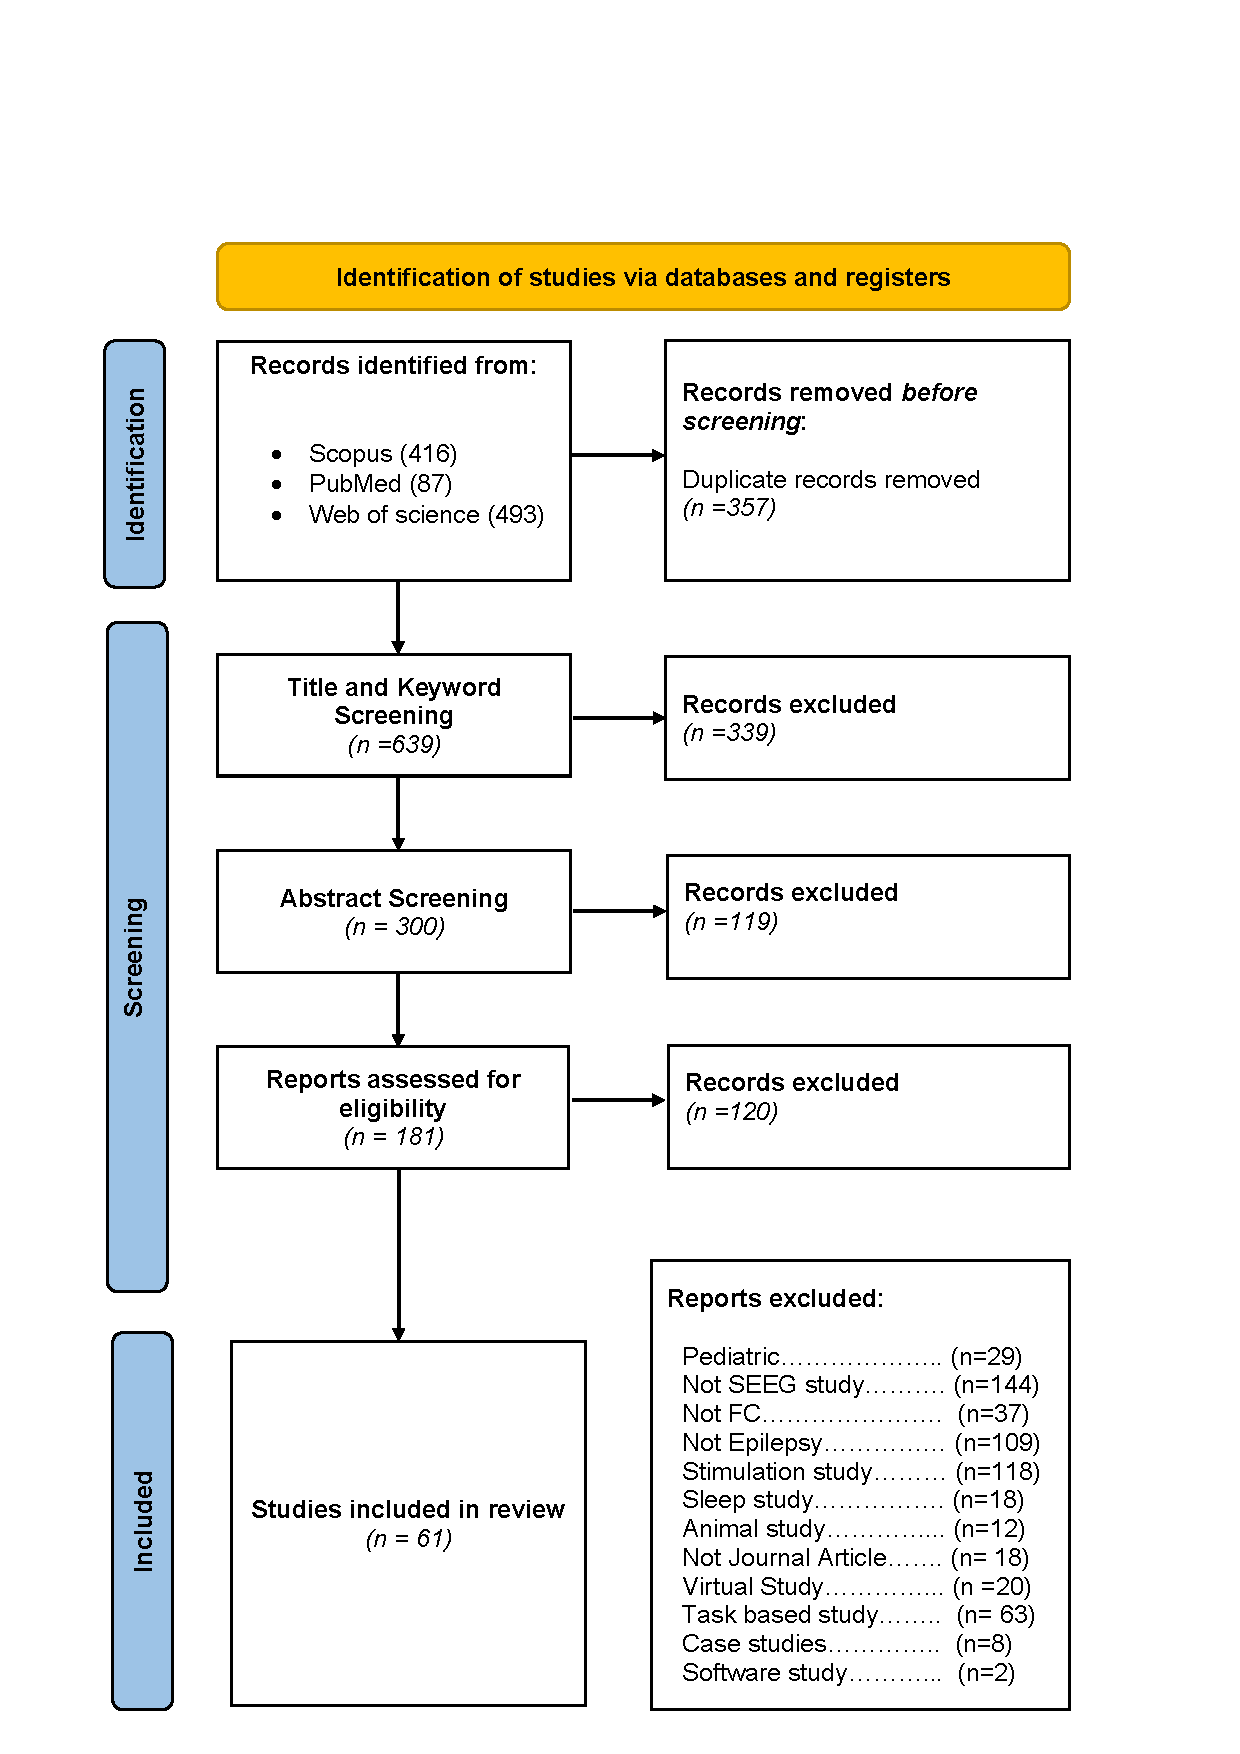
\includegraphics[width=0.8\textwidth]{PRISMA_final.pdf}
  \caption{\textbf{PRISMA 2020 flow diagram of study selection.} Records were
  identified from Scopus ($n=416$), PubMed ($n=87$), and Web of Science
  ($n=493$; total $n=996$). After removal of 357 duplicates, 639 records were
  screened by title and keyword (339 excluded); abstract screening of 300
  records further excluded 119 records; of 181 full-text articles, 120 were excluded,
  yielding 61 included studies.}
  \label{fig:prisma}
\end{figure}



% ============================================
% TABLE 1: FC METHOD OVERVIEW
% ============================================
\begin{landscape}
  \setlength{\LTcapwidth}{\linewidth}
  \fontsize{7pt}{9pt}\selectfont
  \renewcommand{\arraystretch}{1.4}
  \setlength{\tabcolsep}{3pt}
  \begin{longtable}{
>{\raggedright\arraybackslash}p{3cm}
>{\centering\arraybackslash}p{7cm}
>{\centering\arraybackslash}p{2cm}
>{\centering\arraybackslash}p{3cm}
>{\raggedright\arraybackslash}p{7.5cm}
}

%=================================================
% HEADER (FIRST PAGE)
%=================================================
\caption{Summary of Functional Connectivity Analysis Techniques.}
\label{tab:FC_table} \\
\toprule
\textbf{Method} & \textbf{Definition} & \textbf{Range} & \textbf{Complexity} & \textbf{Function}\\
\midrule
\endfirsthead
%=================================================
% HEADER (CONTINUATION PAGES)
%=================================================
\multicolumn{5}{c}{\tablename\ \thetable{} -- \textit{continued}}\\
\toprule
\textbf{Method} & \textbf{Definition} & \textbf{Range} & \textbf{Complexity} & \textbf{Function}\\
\midrule
\endhead
%=================================================
% FOOTERS (empty: each category has its own legend)
%=================================================
\endfoot
\endlastfoot

%========== Category 1: Linear ==========

Pearson Correlation & $r_{xy}=\dfrac{\big\langle\big(x[n]-\bar{x}\big)\big(y[n]-\bar{y}\big)\big\rangle}{\sigma_x\,\sigma_y}$ & [-1,1] & $O(N)$ & Instantaneous linear coupling between two signals.\\[15ex]

Cross-Correlation & $r_{xy}(\tau)=\dfrac{\big\langle\big(x[n]-\bar{x}\big)\big(y[n+\tau]-\bar{y}\big)\big\rangle}{\sigma_x\,\sigma_y}$ & [-1,1] & $O(N)$ & Identifies temporal delays and lead-lag relationships between signals.\\[15ex]

Spectral Coherence & $C_{xy}(f)=\dfrac{\big|\hat{S}_{xy}(f)\big|^{2}}{\hat{S}_{xx}(f)\,\hat{S}_{yy}(f)}$ & [0,1] & $O(N \ log N)$ & Measures consistency of oscillatory interactions at a given frequency.\\[15ex]

Imaginary Coherence & $\mathrm{iCoh}(f)=\Im\!\left\{\dfrac{\hat{S}_{xy}(f)}{\sqrt{\hat{S}_{xx}(f)\,\hat{S}_{yy}(f)}}\right\}$ & [-1,1] & $O(N \ log N)$ & Reduces spurious connectivity caused by volume conduction and common sources.\\[15ex]

Lagged Coherence & $\mathrm{LagCoh}^{2}_{xy}(f)=\dfrac{\Big(\Im\big\{\hat{S}_{xy}(f)\big\}\Big)^{2}}{\hat{S}_{xx}(f)\,\hat{S}_{yy}(f)-\Big(\Re\big\{\hat{S}_{xy}(f)\big\}\Big)^{2}}$ & [0,1] & $O(N \ log N)$ & Estimates delayed interactions while minimizing instantaneous coupling effects.\\*

\multicolumn{5}{@{}l}{\tiny\itshape Linear} \\*

\midrule
\multicolumn{5}{@{}p{22.8cm}@{}}{%
\renewcommand{\arraystretch}{1.1}%
\begin{minipage}[t]{22.8cm}
\tiny
\textbf{Notation}\\[2pt]
\begin{tabular}[t]{@{}ll@{\hspace{4em}}ll@{\hspace{4em}}ll@{\hspace{4em}}ll@{\hspace{4em}}ll@{}}
$x[n]$      & Discrete-time signal $x$                  &    $X(f)$     & Fourier transform of $x[n]$       &    $\hat{S}_{xx}(f)=X(f)X^{*}(f)$         & Auto-spectral density of $x[n]$              \\
$y[n]$      & Discrete-time signal $y$                  &    $Y(f)$     & Fourier transform of $y[n]$       &    $\hat{S}_{xy}(f)=X(f)Y^{*}(f)$         & Cross-spectral density of $x[n]$ and $y[n]$  \\
$\bar{x}$   & Mean of signal $x[n]$                     &    $X^{*}(f)$ & Complex conjugate of $X(f)$       &    $\Re\{\cdot\}$ & Real part             & \\
$\bar{y}$   & Mean of signal $y[n]$                     &    $Y^{*}(f)$ & Complex conjugate of $Y(f)$       &    $\Im\{\cdot\}$ & Imaginary part        &\\
$\sigma_x$  & Standard deviation of signal $x[n]$      &               &                                   &                                           &\\
$\sigma_y$  & Standard deviation of signal $y[n]$      &               &                                   &                                           &\\
\end{tabular}
\end{minipage}%
}\\

\newpage
%========== Category 2: Non-linear ==========

Non-linear Regression & $h_{xy}^{2}(\tau)=1-\dfrac{\displaystyle\sum_{n=1}^{N}\big(y[n+\tau]-g(x[n])\big)^2}{\displaystyle\sum_{n=1}^{N}\big(y[n]-\bar{y}\big)^2}$ & [0,1] & $O(N^2)$ & Quantifies non-linear relationships between signals that are not captured by correlation.\\[15ex]

Phase-Locking Value & $\mathrm{PLV}=\Bigg|\dfrac{1}{N}\displaystyle\sum_{n=1}^{N}\exp^{\,j(\phi_{x}[n]-\phi_{y}[n])}\Bigg|$ & [0,1] & $O(N)$ & Measures consistency of phase differences across time or trials.\\[15ex]

Phase-Lag Index & $\mathrm{PLI}=\left|\dfrac{1}{N}\displaystyle\sum_{n=1}^{N}\mathrm{sgn}\big(\sin(\phi_{x}[n]-\phi_{y}[n])\big)\right|$ & [0,1] & $O(N)$ & Measures consistent non-zero phase leads/lags while reducing volume-conduction effects.\\[15ex]

Mutual Information & $I(X;Y)=\displaystyle\sum_{x,y}p(x,y)\,\log\frac{p(x,y)}{p(x)\,p(y)}$ & [0,$\infty$) & $O(NB) - O(N^2)$  & Captures both linear and non-linear shared information between signals.\\[15ex]

Relative Entropy & $D_{\mathrm{KL}}\big(p\,\|\,q\big)=\displaystyle\sum_{x}p(x)\,\log\frac{p(x)}{q(x)}$ & [0,$\infty$) & $O(B)$ after histogram estimation & Quantifies difference between signal probability distributions or brain states.\\*

\multicolumn{5}{@{}l}{\tiny\itshape Non-linear} \\*

\midrule
\multicolumn{5}{@{}p{22.8cm}@{}}{%
\renewcommand{\arraystretch}{1.1}%
\begin{minipage}[t]{22.8cm}
\tiny
\textbf{Notation}\\[2pt]
\begin{tabular}[t]{@{}ll@{\hspace{2.5em}}ll@{\hspace{2.5em}}ll@{}}
$\phi_x[n]$                 & Instantaneous phase of signal $x[n]$        & $p(x)$          & Marginal probability distribution of $X$    & $p(x,y)$    & Joint probability distribution of $X$ and $Y$ \\
$\phi_y[n]$                 & Instantaneous phase of signal $y[n]$        & $p(y)$          & Marginal probability distribution of $Y$    & $q(x)$      & Reference probability distribution \\
$\mathrm{sgn}(\cdot)$       & Sign function ($+1$, $0$, or $-1$)          & $N$             & Number of samples (or observations) & & \\
$g(\cdot)$                  & Optimal nonlinear regression function relating $x[n]$ to $y[n+\tau]$ & $f$  & Frequency & & \\
\end{tabular}
\end{minipage}%
}\\
\newpage

%========== Category 3: Directed ==========

Granger Causality & $F_{x\to y}=\ln\dfrac{\mathrm{var}\big(\varepsilon_y^{\mathrm{red}}\big)}{\mathrm{var}\big(\varepsilon_y^{\mathrm{full}}\big)}$ & [0,$\infty$) & $O(M^3p^2 + MNp)$ & Determines whether past activity in one signal improves prediction of another signal.\\[15ex]

Directed Transfer Function & $\gamma_{ij}^2(f)=\dfrac{\big|H_{ij}(f)\big|^{2}}{\displaystyle\sum_{m=1}^{M}\big|H_{im}(f)\big|^{2}}$ & [0,1] & $O(M^3F)$ after MVAR fit & Estimates frequency-specific information flow within a network based on MVAR models.\\[15ex]

Partial Directed Coherence & $\pi_{ij}^2(f)=\dfrac{\big|\bar{A}_{ij}(f)\big|^{2}}{\displaystyle\sum_{m=1}^{M}\big|\bar{A}_{mj}(f)\big|^{2}}$ & [0,1] & $O(M^3F)$ after MVAR fit &  Identifies direct causal influences between nodes while accounting for other network connections.\\[15ex]

Transfer Entropy & $TE_{x\to y}=\sum_{y_{n+1},\,y_n^{(k)},\,x_n^{(l)}}p\!\left(y_{n+1},y_n^{(k)},x_n^{(l)}\right)\log\frac{p\!\left(y_{n+1}\mid y_n^{(k)},x_n^{(l)}\right)}{p\!\left(y_{n+1}\mid y_n^{(k)}\right)}$ & [0,$\infty$) & $O(N^2) - O(N^3)$ & Model-free directed information transfer; Quantifies how much the past of one signal improves prediction of another.\\*

\multicolumn{4}{@{}l}{\tiny\itshape Directed} \\*
\midrule
\multicolumn{5}{@{}p{22.8cm}@{}}{%
\renewcommand{\arraystretch}{1.3}%
\begin{minipage}[t]{22.8cm}
\tiny
\textbf{Notation}\\[2pt]
\begin{tabular}[t]{@{}ll@{\hspace{1.5cm}}ll@{\hspace{1.5cm}}ll@{\hspace{1.5cm}}ll@{}}
$\varepsilon_y^{\mathrm{red}}$  & Reduced-model prediction error  &  $H_{ij}(f)$ & MVAR transfer function, $j \to i$                            &  $A_r$  & MVAR coefficients at lag $r$    &  $M$ & Number of network nodes   \\
$\varepsilon_y^{\mathrm{full}}$ & Full-model prediction error     &  $\bar{A}_{ij}(f)$ & $\big[I-\sum_{r=1}^{p}A_r e^{-j2\pi fr}\big]_{ij}$     &  $p$    & MVAR model order               &  $I$ & Identity matrix           \\
$y_n^{(k)}$ & Past $k$ samples of $y$ & $x_n^{(l)}$ & Past $l$ samples of $x$ \\ 
\end{tabular} \\[1pt]
\begin{tabular}[t]{@{}ll@{}}
$p(y_{n+1},y_n^{(k)},x_n^{(l)})$ & Joint probability distribution of the future state of \(Y\), the past \(k\)-sample history of \(Y\), and the past \(l\)-sample history of X \\
$p(y_{n+1}\mid y_n^{(k)})$    & Conditional probability of the future state $y_{n+1}$ given the past $k$ observations of $y$ \\
$p(y_{n+1}\mid y_n^{(k)},x_n^{(l)})$    & Conditional probability of the future state $y_{n+1}$ given the past histories of both $y$ and $x$
\end{tabular}
\end{minipage}%
}\\

  \end{longtable}
\end{landscape}


\end{document}
